\chapter{Grundlagen}
\label{sec:grundlagen}

\section{Grid Fins als Steuerelement von Flugkörpern im Hyperschall}
\subsection{Aufbau}
In der simpelsten Konfiguration bestehen Grid Fins aus einem äußeren Rahmen, der die innere Struktur von sich kreuzenden planaren Flächen stützt. Dieser einfache Aufbau gewährt hohe Stabilität bei vergleichsweise geringem Gewicht und lässt sich mittels 5 Parameter, wie in Abbildung \ref{abb_parameter} zu sehen, beschreiben. Die Wanddicke $d$ kann sich für den Rahmen ($d_R$) von der für das Gitter ($d_G$) unterscheiden. Aber auch innerhalb dieser Einteilung kann der Wert variieren, so ist häufig die Wandstärke in der Nähe der Einspannung zu erhöhen, um die dort auftretenden höheren Beanspruchungen zu ertragen. Ein umrahmtes Segment des Gitters wird als Zelle bezeichnet und ihre Dimension kann mit die Zellgröße $g$ beschrieben werden. Die Ausmaße der Grid Fins wird maßgeblich durch die Spannweite $b$ und die Höhe $h$ bestimmt. Die Querschnittsfläche $A$ steht in der Ausgangsstellung senkrecht zur Anströmung und wird vom Rahmen begrenzt. Normal zu dieser Fläche steht die Sehne mit einer im Vergleich zur planaren Finne deutlich kürzeren Länge $s$.\\
\begin{figure}[h]
	\centering
	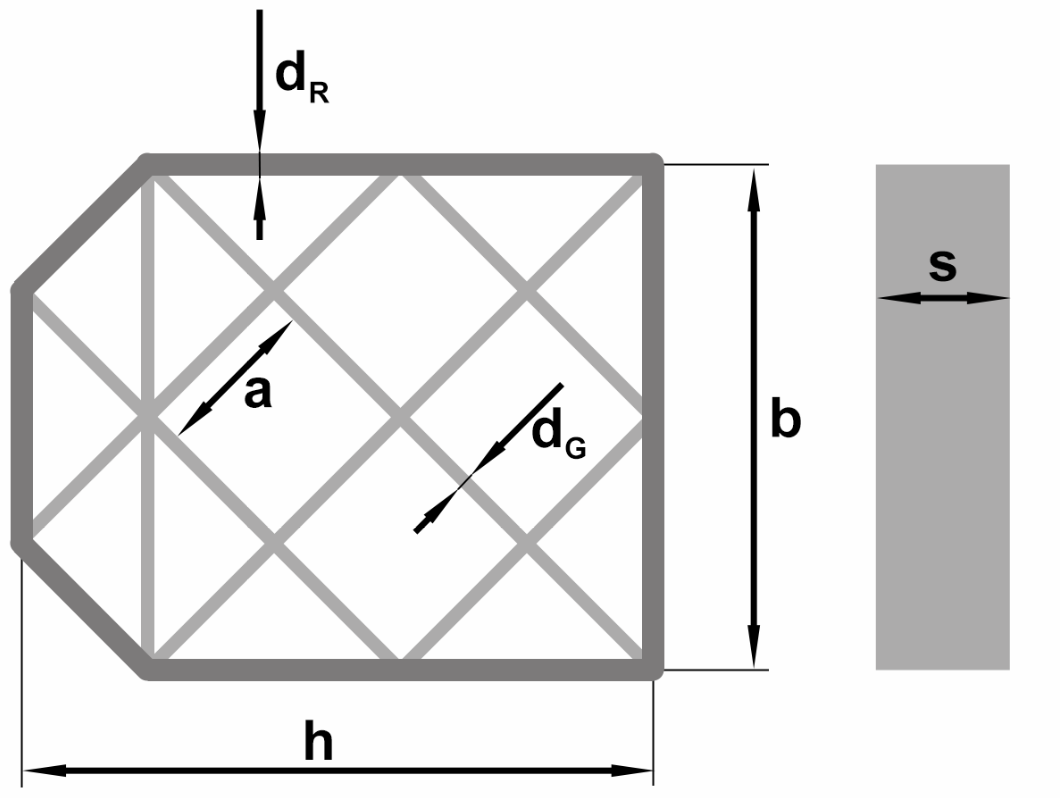
\includegraphics[width=0.6\textwidth]{Parameter.png}
	\caption{Aufbau eines einfachen Grid Fins}
	\label{abb_parameter}
\end{figure}\\
Grid Fins müssen nicht starr an einem Körper befestigt werden, sondern können um mehrere Achsen drehbar sein. Um sie für den Transport kompakt zu lagern, lassen sie sich an den Körper anlegen. Der Klappwinkel $\Lambda$ beschreibt den Ausschlag um eine den Körper an der Anbringung tangierende Achse. Ein Klappwinkel von $0°$ entspricht hierbei den normalen in den Strömung ragenden Zustand und $90°$ den eingeklappten. Zur Steuerung lassen sich die Grid Fins um eine Achse, die senkrecht aus dem Körper durch die Mitte des Grid Fins zeigt, verstellen. Ein Steuerwinkel von $\eta = 0°$ ist auch hier wieder die Ausgangsstellung, die Sehne ist parallel zur Strömung. Bei $\eta = 90°$ würde also die Seitenkante zur Anströmung zeigen, die Querschnittsfläche $A$, also das Gitter, wird nicht durchströmt.\\
\begin{figure}[h]
	\centering
	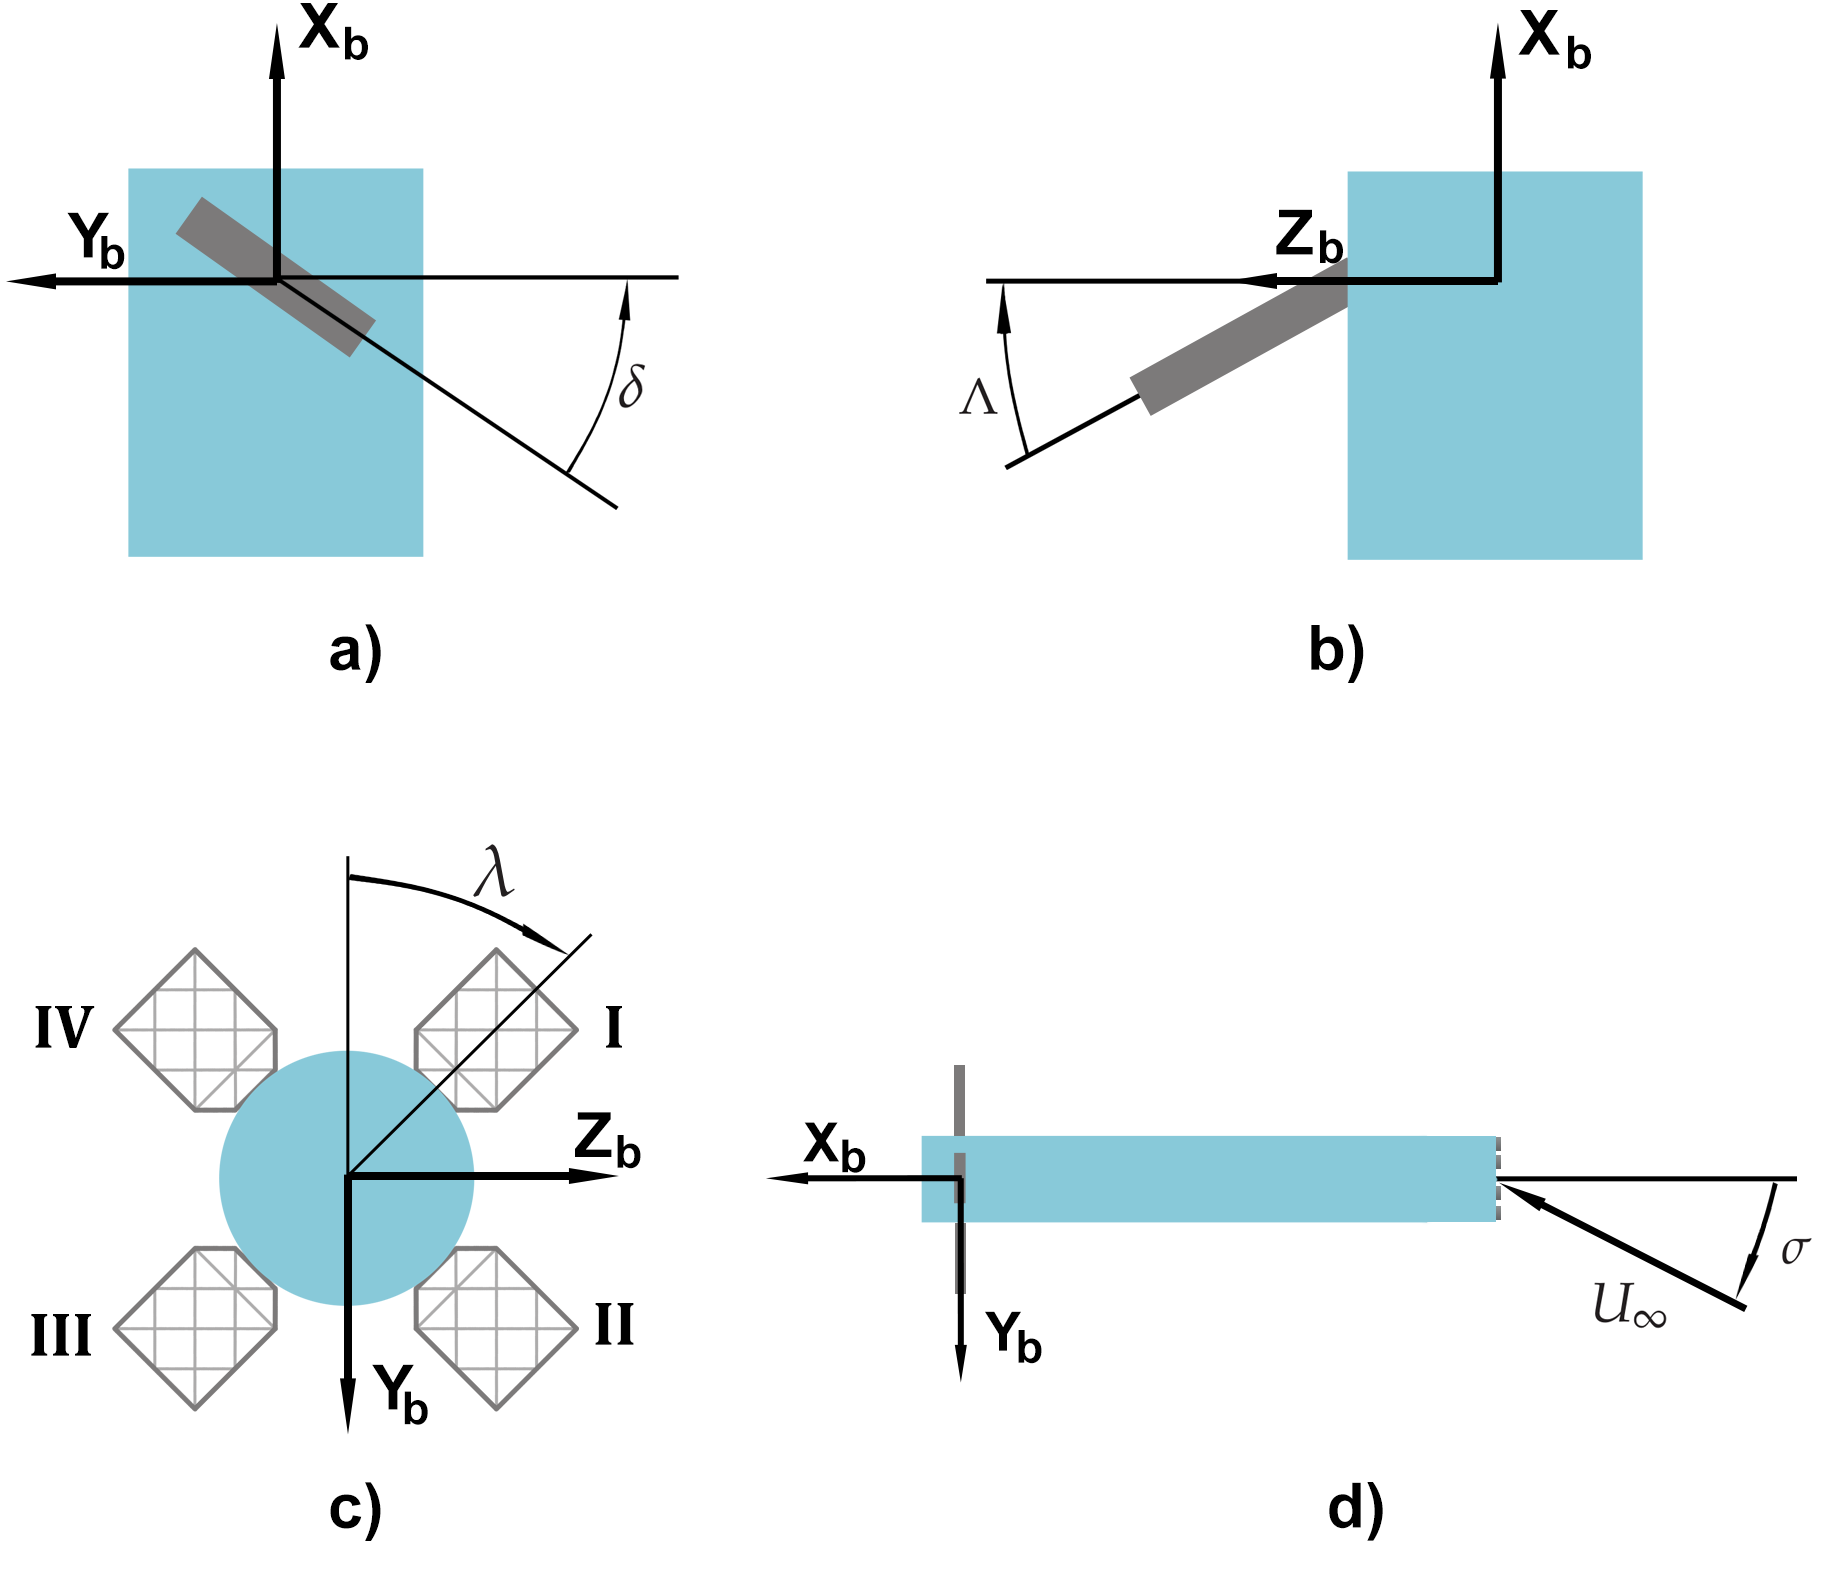
\includegraphics[width=0.8\textwidth]{Winkel.png}
	\caption{Winkel zur Beschreibung der Orientierung der Grid Fins zum Körper\\a) Steuerwinkel, b) Klappwinkel, c) Drehwinkel, d) Anstellwinkel des Körpers}
	\label{abb_winkel}
\end{figure}\\
Um die Aerodynamik zu untersuchen reichen diese Winkel nicht aus, da die Anströmung nicht parallel zur Rakete liegen muss. Der Anstellwinkel des gesamten Modus $\sigma$ setzt sich unter realen Bedingungen aus dem Schiebewinkel und dem Bahnneigungswinkel, unter Vernachlässigung des Windes, zusammen. Für die in dieser Arbeit durchgeführten Untersuchungen ist eine solche Aufteilung aber irrelevant. Damit aber keine Informationen und somit Genauigkeit verloren geht, wird stattdessen die Orientierung der Grid Fins auf dem Umfang betrachtet. Verwendet wird hier eine Anordnung von vier gleichmäßig verteilten Steuerelementen. Das Koordinatensystem ist so definiert, dass es seinen Ursprung genau in der Mitte dieser Konfiguration hat und die positive X-Achse zur Spitze des Flugkörpers, also entgegen der Anströmung, zeigt. Bei $\sigma \neq 0$ zeigt auch die Y-Achse einem Anteil der Strömung entgegen. Die Z-Achse ist folglich nach den Rechtssystem orthogonal zu den anderen beiden ausgerichtet. Um nun die Orientierung der Grid Fins um die X-Achse herum beschreiben zu können wird der Rollwinkel $\lambda$ eingeführt. Wenn eine '+'-Konfiguration vorliegt, befinden sich die einzelnen Finnen auf den Koordinatenachsen (X, Y) und der Rollwinkel ist gleich null. Im Gegensatz dazu bei der 'x'-Konfiguration sind sie um einen Winkel von $\lambda = 45°$ verdreht. Der Anstellwinkel $\alpha$, den ein einzelner Grid Fin erfährt, lässt sich aus dem Anstellwinkel des Körpers und, in Abhängigkeit vom Rollwinkel und welcher der Finnen überhaupt betrachtet wird, aus dem Klapp- und Steuerwinkel bestimmen.
\subsection{Strömung durch Grid Fins}

\subsection{Verhalten im transsonischen Bereich}
\subsection{Aerodynamische Beiwerte und Vergleich zu planaren Finnen}
\subsection{Bisherige Implementierung/ Grid Fin Varianten}

\section{Wiedereintrittsbedingungen}

\section{Das Air-Launchsystem Valkyrie}

